\input{dfki.defs}


\usepackage[hidelinks]{hyperref}

\title[Simulation in Robotics]{Lecture 3 - Simulation of Techniques and Tools}
\author{Julius Martensen}
\date{\today}

\begin{document}


\frame{\titlepage}

\section{A holistic perspective}

\frame{
	\frametitle{Robotics - An Interdisciplinary Science}

	\begin{figure}
		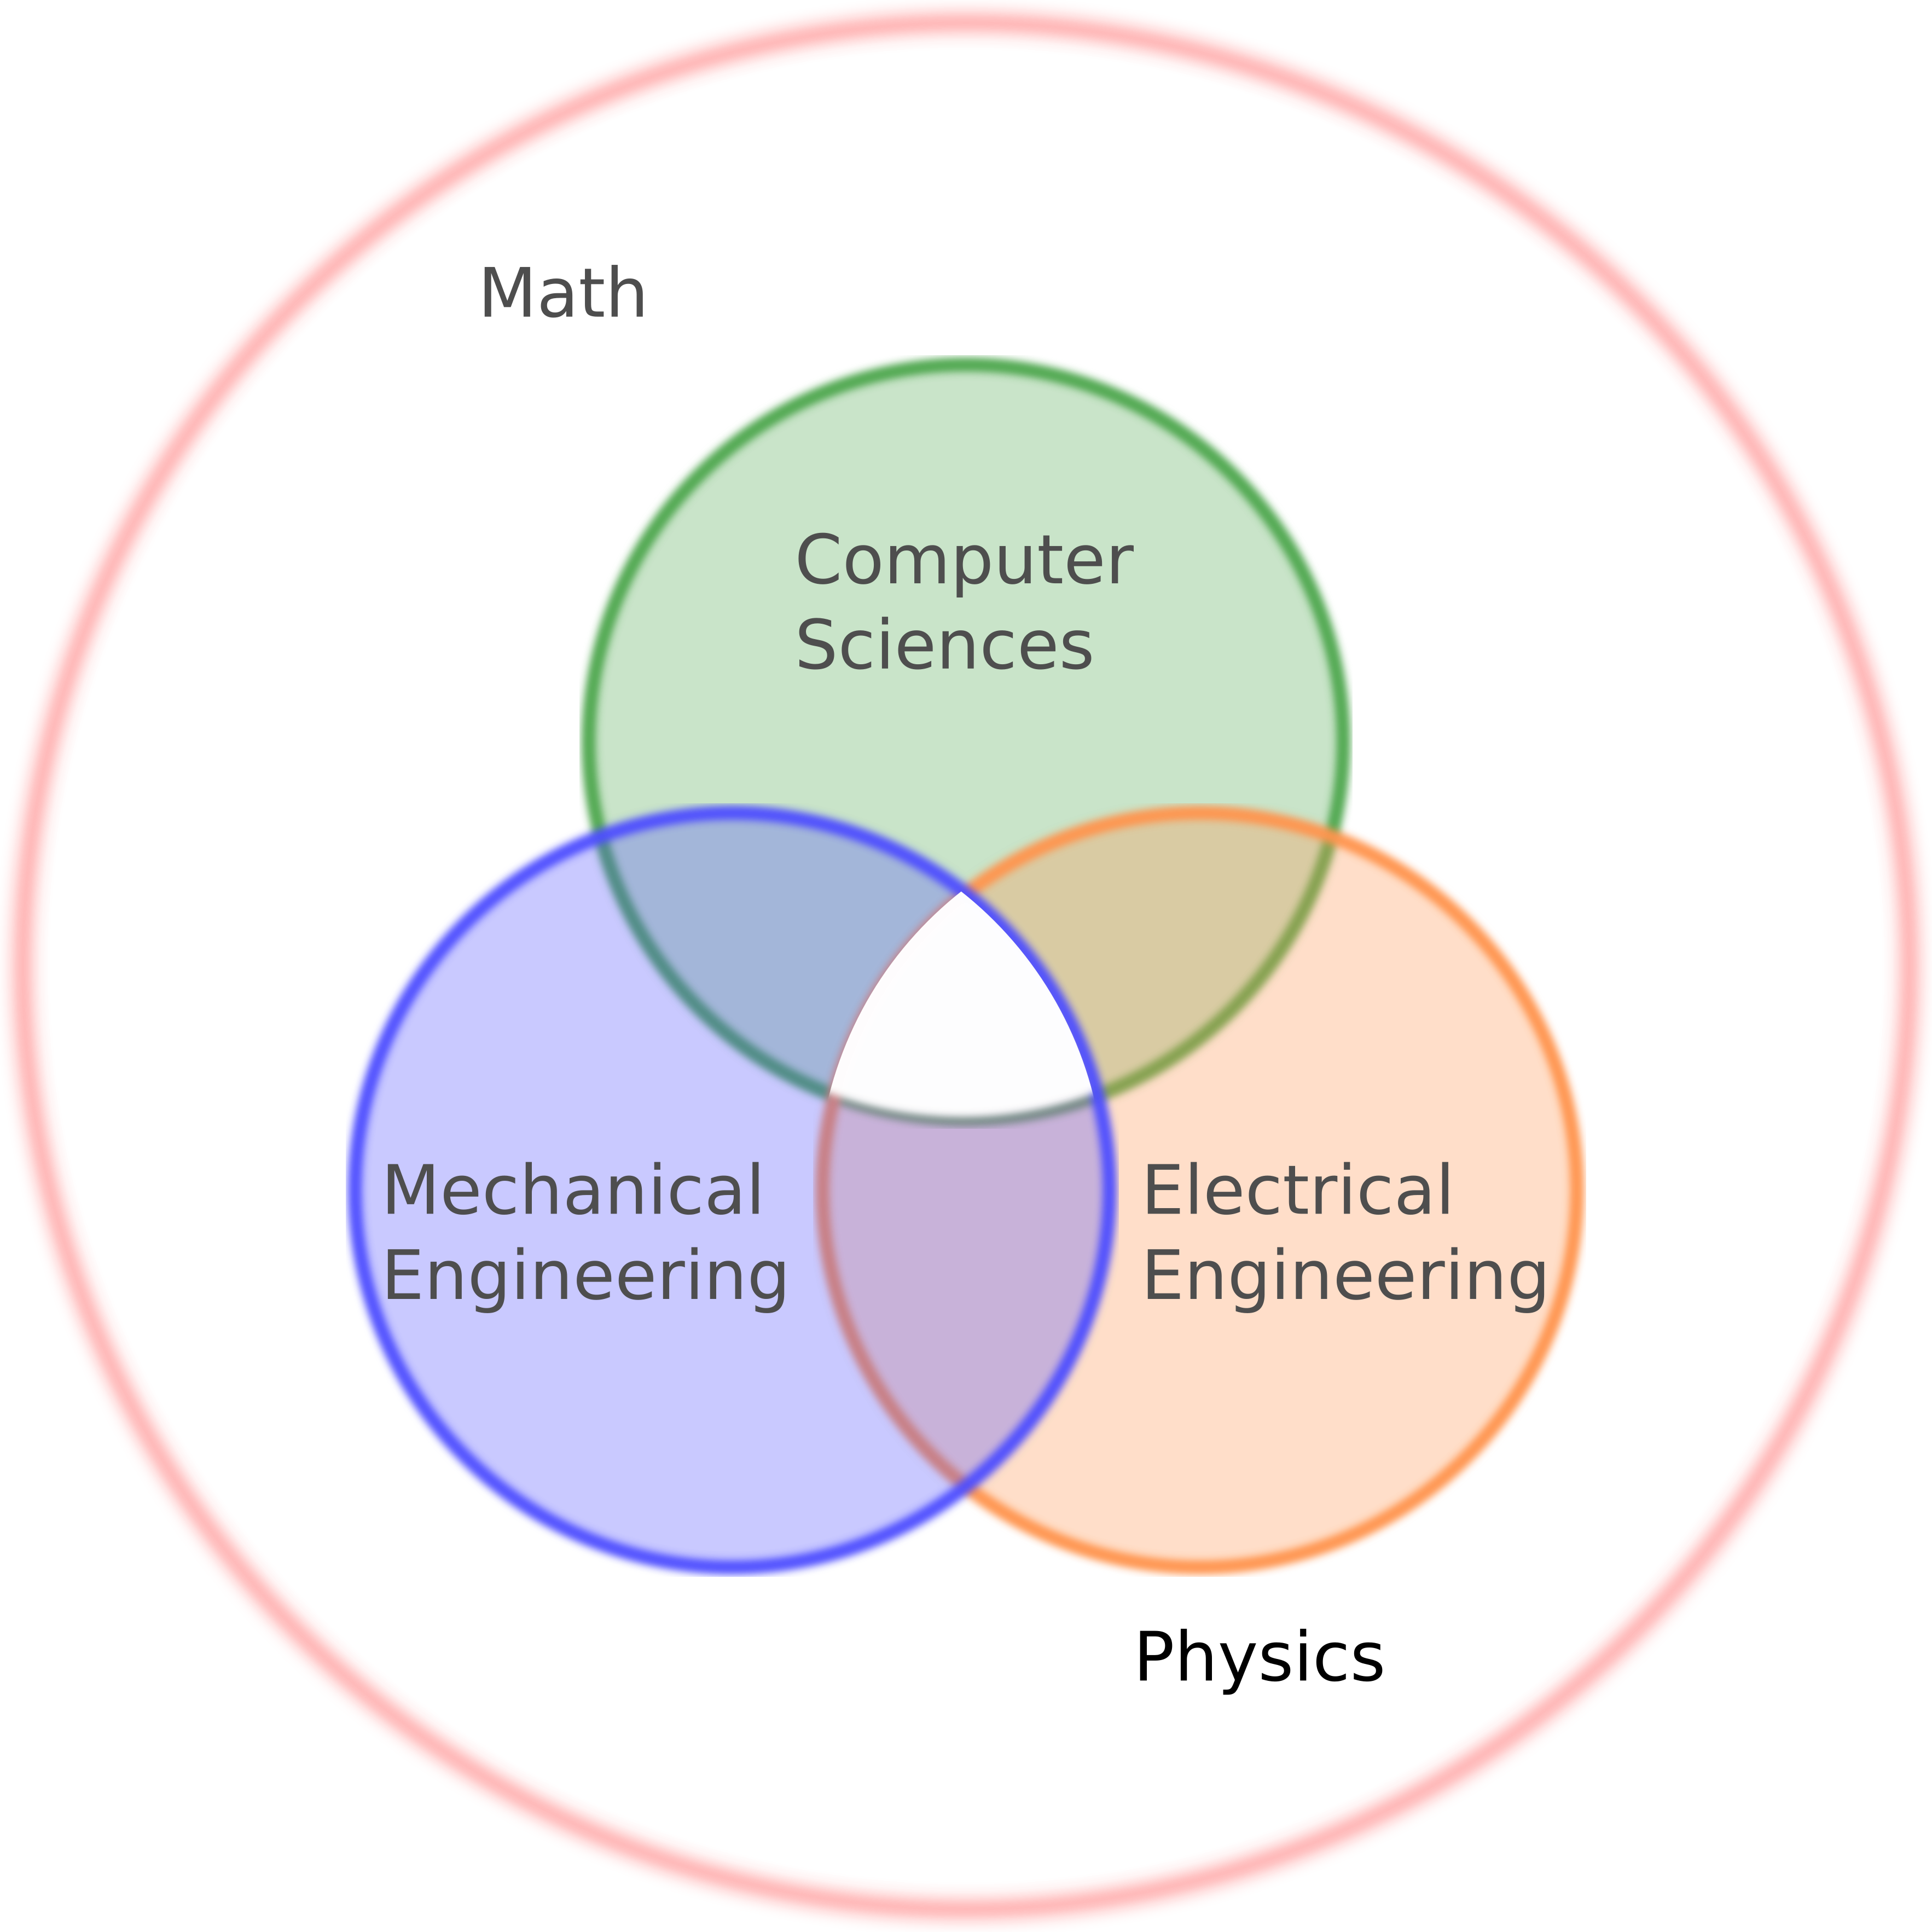
\includegraphics[width = 0.5\textwidth]{./pics/robotics_motivation.png}
	\end{figure}

}

\frame{
	\frametitle{Modeling Approaches}
	\begin{column}{0.5\textwidth}
		Bottom Up
		\begin{itemize}
			\item A model consists of submodels
			\item Every parameter is considered
			\item High physical accuracy
		\end{itemize}
	\end{column}%
	\begin{column}{0.5\textwidth}
		Top Down
		\begin{itemize}
			\item A model consists of an input-output behavior
			\item A subset of parameters are needed
			\item Efficient simulation
		\end{itemize}
	\end{column}%
}

\frame{
	\begin{column}{0.5\textwidth}
		Bottom Up
		\begin{itemize}
			\item (Low Level) Controller Design
			\item Learning more than I/O relations
			\item More "realistic" behavior
		\end{itemize}
	\end{column}%
	\begin{column}{0.5\textwidth}
		Top Down
		\begin{itemize}
			\item (High level) controller design
			\item Learning basic I/O relations
			\item Visual behavior / Gaming
		\end{itemize}
	\end{column}
}

\section{Opportunities and Limitations}

\frame{
	\frametitle{Soft Body Dynamics}
	\begin{column}{0.5\textwidth}
		\begin{itemize}
			\item<1-> Connect \textbf{each} node of a mesh with a spring damper system
			\item<2-> Huge effort from numerical point of view
			\item<3-> \href{https://youtu.be/9sh-D0nejUY}{Examples}
		\end{itemize}

	\end{column}
	\begin{column}{0.5\textwidth}
	\begin{figure}
		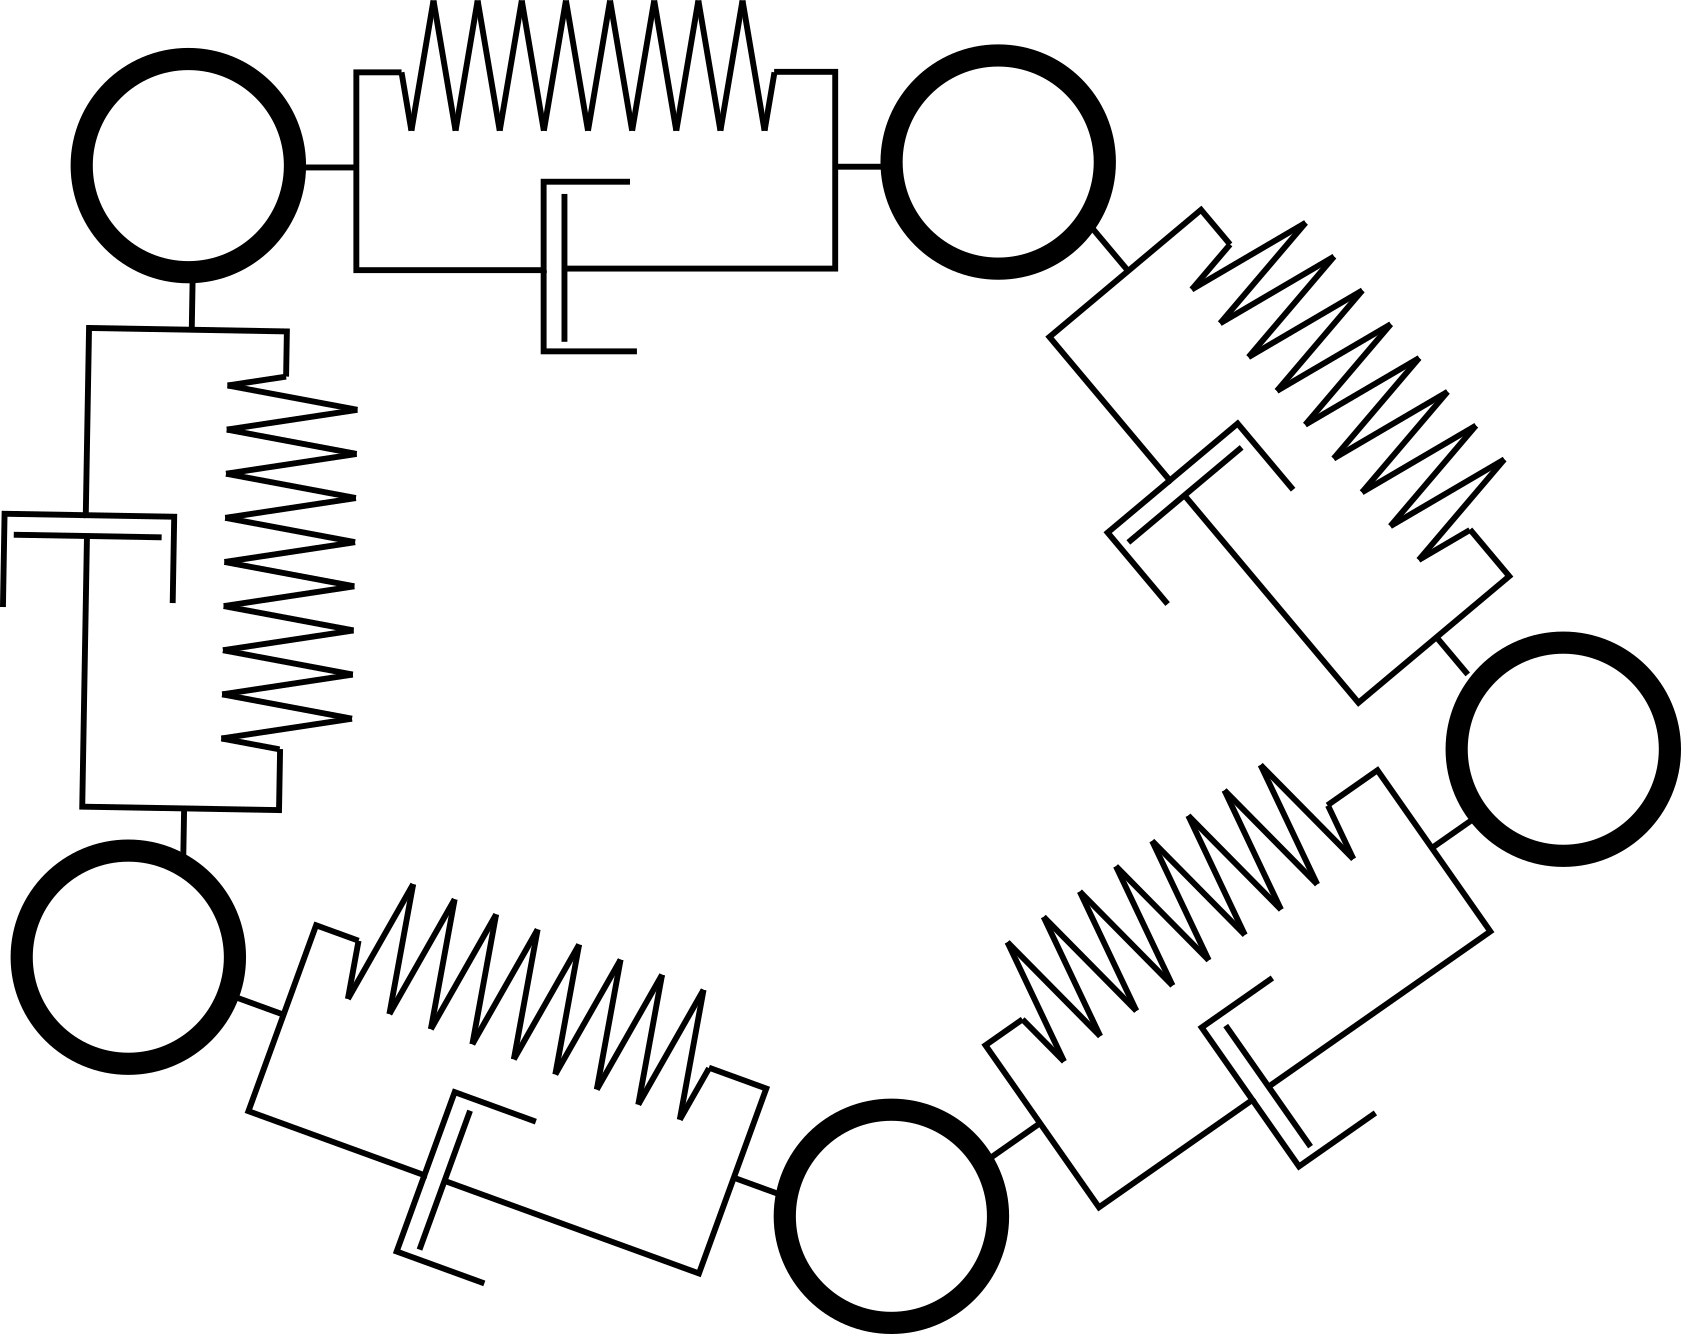
\includegraphics[width = 0.9\textwidth]{./pics/soft_body.png}
	\end{figure}
	\end{column}
}

\section{Caveats of Robotic Simulation}

\frame{
	\frametitle{Good Questions}
	\begin{column}{0.5\textwidth}
		\begin{itemize}
			\item<1-> How to model joint clearance?
			\item<3-> How to make objects grippable?
			\item<5-> Avoid self collision?
		\end{itemize}
	\end{column}
	\begin{column}{0.5\textwidth}
		\begin{itemize}
			\item<2-> Using CFM and ERP.
			\item<4-> Enable pairings of object and destroyable fixed links
			\item<6-> If needed, use collision layers.
		\end{itemize}
	\end{column}
}


\frame{
	\frametitle{Problem Abstraction}

	\begin{exampleblock}<1->{Description}
		Model a factory worker which can step in the working cell of a robot.
		The robot is able to identify a worker via visual detection. \newline
	\end{exampleblock}

	\begin{alertblock}<2->{Abstraction I}
		Model a visual of the factory worker that is able to "walk" in the simulation.
	\end{alertblock}

	\begin{alertblock}<3->{Abstraction II}
		Model a visual of the factory worker that is able to change its position smoothly.
	\end{alertblock}

}

\frame{
	\frametitle{Using the Right Tools}

	\begin{exampleblock}<1->{Description}
		Estimate the forces acting on each joint during a given walking gait.
	\end{exampleblock}

	\begin{alertblock}<2->{Abstraction}
			High accuracy simulation of a robots lower body.
	\end{alertblock}

	\begin{block}<3->{Suitability}
		Is a rigid body simulator sufficient for the task?
	\end{block}

}


\frame{
	\frametitle{"Nonphysical" Models}

	\begin{exampleblock}<1->{Description}
		Model a factory worker which walks around naturally.
	\end{exampleblock}

	\begin{alertblock}<2->{Abstraction}
		Give a model a walking like behavior.
	\end{alertblock}

	\begin{block}<3->{Requirements}
		Ray Tracing: Detects objects in front of it. \\
		Target Generator: Creates a (reachable) target.
	\end{block}
}


\frame{
	\frametitle{"Nonphysical" Models}

	\begin{exampleblock}{Description}
		Model a factory worker which walks around naturally.
	\end{exampleblock}

	\begin{alertblock}{Abstraction}
		Give a model a walking like behavior.
	\end{alertblock}

	\begin{block}<2->{Solutions}
		Look at gaming AI. Many algorithms are present.\\
		Maybe a simple control strategy is sufficient?
	\end{block}

}


\frame{
	\frametitle{Nearly Physical Models}
	\begin{exampleblock}<1->{Task}
		Model a current for underwater simulations.
	\end{exampleblock}

	\begin{alertblock}<2->{Solution}
		Create a vectorfield of current forces and add some degree of randomness!
	\end{alertblock}

}
\section{Co-Simulation of Models}

\frame{

	\begin{center}
		{\Huge Live Coding}
	\end{center}
}

\section{Sensor Modeling}

\frame{
	\frametitle{Model of an IMU}

	\begin{exampleblock}<1-3>{Task}
		Measure the acceleration and rotational velocity at a given frame.
	\end{exampleblock}

	\begin{figure}
		\includegraphics<2>[width = 0.5\textwidth]{./pics/IMU.png}
	\end{figure}

	\begin{alertblock}<3>{Equations}
	\begin{align*}
		^{I}\textbf{a} &= ^{I}\textbf{R}_{0} ^{0}\textbf{a} + ^{I}\textbf{T}_{0} ^{0}\textbf{w} \\
		^{I}\textbf{w} &= ^{I}\textbf{R}_{0} ^{0}\textbf{w}
	\end{align*}

	\end{alertblock}


}

\section{Common Simulationtools}

\frame{
	\frametitle{Gazebo}
	\href{https://youtu.be/SK5GuC1jgg8}{Gazebo Overview}
}

\frame{
	\frametitle{V-Rep}
	\href{https://youtu.be/gBYqOBdIcaY}{V-Rep Overview}
}


\frame{
	\frametitle{OpenModelica}

	\begin{center}
		{\Huge Live Demonstration}
	\end{center}
}


\end{document}
